\documentclass[]{article}
\usepackage{graphicx}

\begin{document}

%%%%%%%%%
\section*{Population Genetics}

\begin{enumerate}
\item What’s the highest possible frequency of heterozygotes at a single biallelic locus at HWE?

\item The frequency of A1 in a population is 0.7.  A troll eats half the homozygous A1A1 individuals, then leaves.  After one generation of completely random mating, is the population at HWE?

\item  In a population at Hardy-Weinberg Equilibrium (HWE) at the A locus, there are six times as many heterozygous A1A2 individuals as homozygous A2A2 genotypes.  What is the frequency of A1?

\item The frequency of the R allele (at a locus with alleles R and r) in a population is 0.4.  If you sample 500 individuals from this population, what is the frequency of the rr genotype? 

\item  In an infinite size diploid neutral population mating randomly with frequency of the MM genotype of 4\%, what is the frequency of the m allele (the locus is biallelic)?

\item  Can genetic drift lead to evolution?  Why or why not?

\item Farmer Jones is trying to eliminate a recessive dwarf allele at the dwarfus locus from his pea crop. In 2010, his fields yielded 9\% dwarf plants. You may assume that his population in 2010 is in HWE. When planting his 2011 crop, the farmer used only the seeds from the tall plants of the previous year. Tall (D) is dominant to dwarf (d). If there is no further selection, what do you predict will be the frequency of dwarf pea plants in the 2012 crop?

\end{enumerate}

%%%%%%%%%
\section*{Gene Expression}
\begin{enumerate}
\item  If I told you that a mutant had a fully functional copy of the mutant gene, with no evidence of mutations in the coding sequence or the promoter, but cDNA for the gene was almost never observed, what mechanisms could explain this result?
\item The transcription of gene TTFN (terrible transcription factor nine) is activated when two other transcription factors (A and B) interact to recruit a co-activator X. A,B, and X combine to create an enhanceosome upstream of TTFN.  Draw a diagram of the interaction between these genes during transcription.   
\item You suspect that a gene is downregulated due to epigenetic modification. Explain how you would show this.
\end{enumerate}

%%%%%%%%%
\section*{Genomics}
\begin{enumerate}
\item  What is the fate of most gene duplicates?


\item Given the tree in figure \ref{fig:TREE} for a gene family in the species chimera, dragon, unicorn, dolphin, and mermaid, answer the following questions:
\begin{enumerate}
%\item If I create a nonsense mutation in dragon1, is it likely to have an effect? Why or why not?
\item Is chimera2 a paralog or ortholog of chimera1?
\item Is chimera2 and ortholog or paralog of dolphin1?
\item What is a likely explanation for why there is only one copy of the gene in mermaid?
\item If dragon1 is expressed in the wings and dragon2 is expressed in the tail, but chimera2 is expressed throughout the body, what kind of process explains the extra copies in dragon?
\end{enumerate}

\begin{figure}[here]
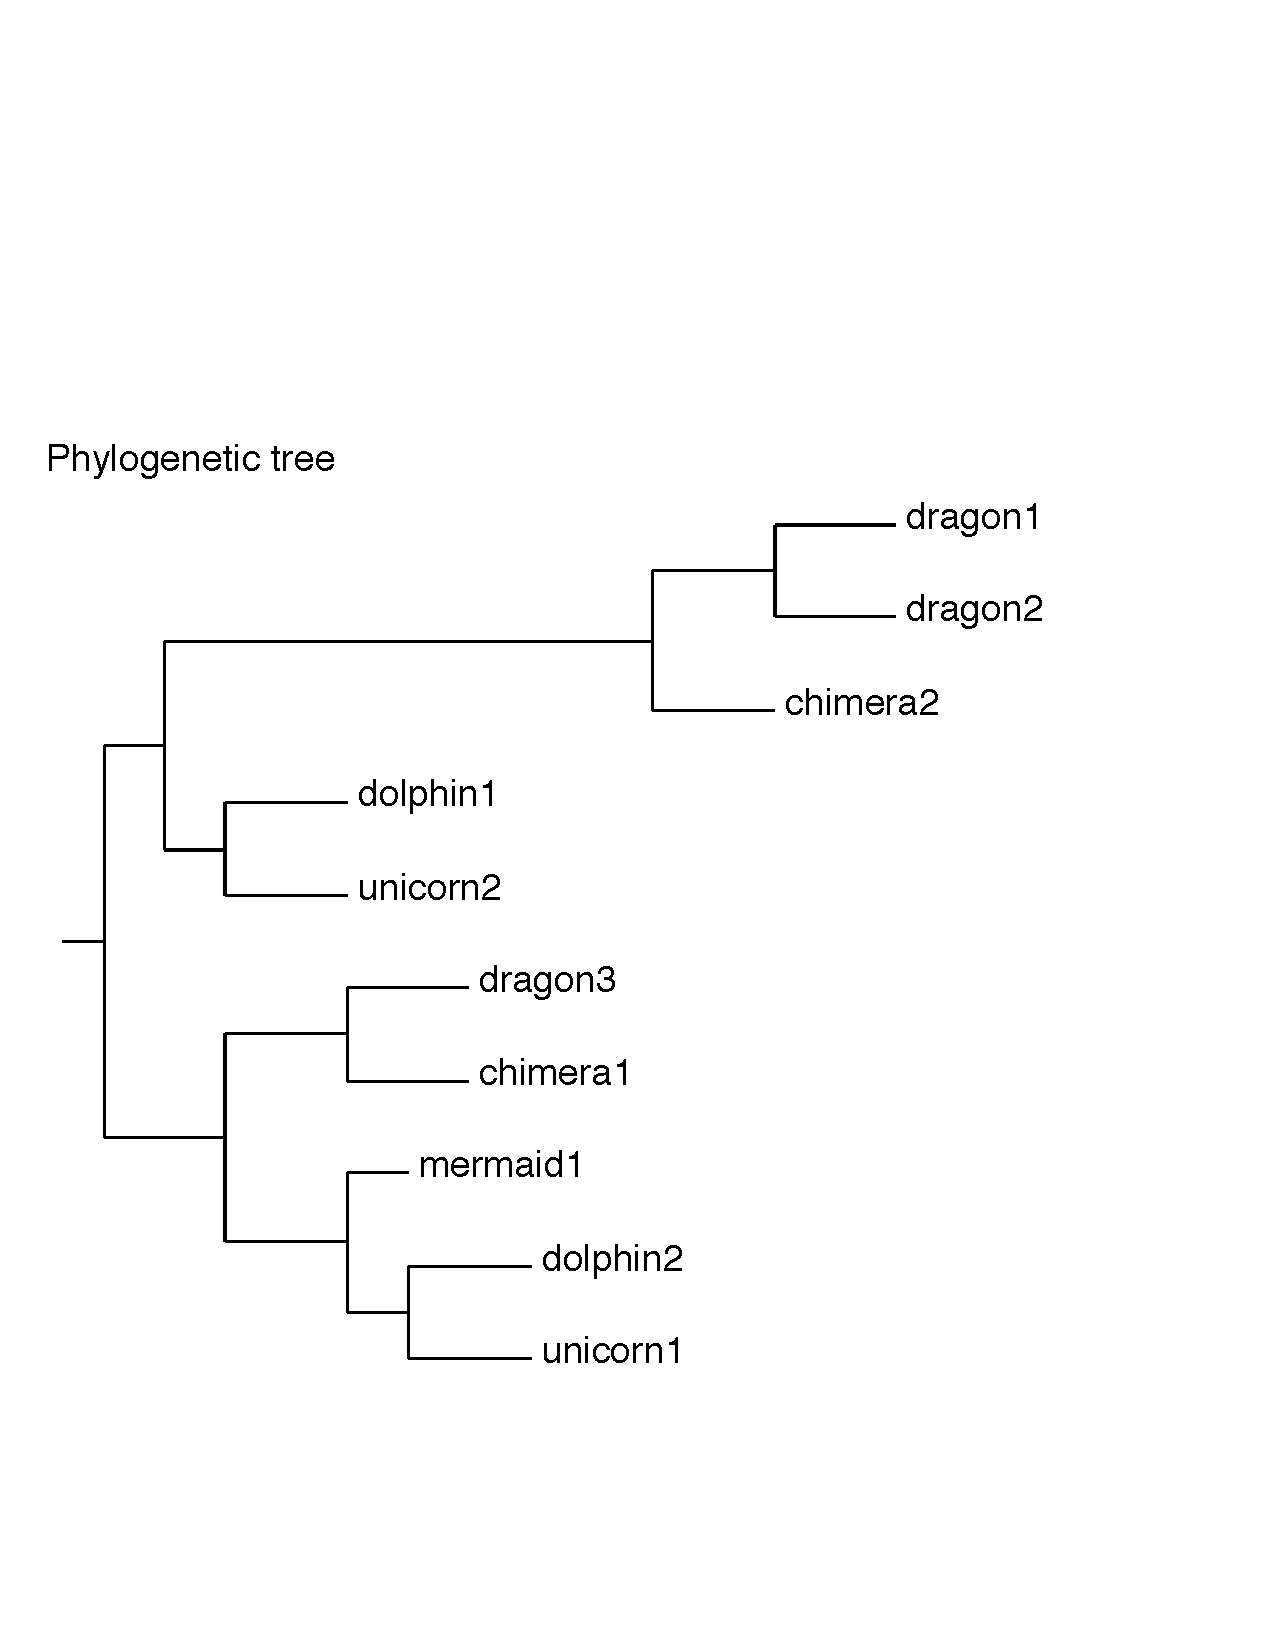
\includegraphics[width=12cm]{faketree.pdf}
\caption{A phylogenetic tree of a fake gene family}
\label{fig:TREE}
\end{figure}
\pagebreak

\item What is synteny and why is it useful?
\item Maize is the second largest plant genome sequenced to date. Given how easy it is to produce sequence data, why haven’t other large genomes been sequenced and assembled?
\end{enumerate}

%%%%%%%%%
\section*{Transposable Elements}
\begin{enumerate}
\item Which class of TEs would you expect to make up the largest part of the genome in plants? How about in \emph{Drosophila}? Why?
\item The maize gene FLX (fluxocapacitor) makes corn kernels sprout puffy white hair (like Christopher Lloyd). Near FLX is a nonautonomous Ds element. If I cross a plant homozygous for functional FLX (FLX+) and presence of the Ds (Ds+) with an inbred plant that has nonfunctioning FLX, no Ds, but an active autonomous Ac element. Draw the phenotype of each parent and the phenotype and genotype of some possible progeny.
\end{enumerate}

\end{document}
